\section{问题重述}

随着"双碳"战略的深入推进，新能源大规模并网消纳难的问题日益凸显\cite{ref2}。绿电直连项目作为促进新能源就近消纳的新路径，通过将风电、光伏等清洁能源直接供给园区内制氢、制氨等高耗能负荷，实现了"绿电—绿氢—绿氨"一体化生产\cite{ref3}。国家发展改革委、国家能源局对绿电直连项目提出了三项核心指标要求：新能源自发自用电量占总可用发电量比例大于60\%、总用电量绿电比例大于30\%、新能源上网电量比例小于20\%。

本题研究一个典型的绿电直连制氢氨园区，该园区包含碱性电解槽（ALKEL，10~MW）、质子交换膜电解槽（PEMEL，10~MW）、合成氨装置（0.75~MW）、风电（40~MW）、光伏（64~MW）及常规电负荷（峰值6~MW）。园区初始制氨产能为36吨/日，产能扩容时配套设备功率线性同步提升。风光发电具有强随机波动性，给定6种风电和4种光伏出力场景，组合形成24种运行工况。需要依次解决以下四个核心问题：

问题一要求在电解槽与合成氨装置满负荷连续运行条件下，计算典型日的功率平衡关系和各项绿电直连指标，分析指标是否满足政策要求。问题二将制氨产能扩至72吨/日，在电氢氨装置仅有全额开机和停机两种运行方式的约束下，寻找使吨氨成本最低的离散生产时段安排方案。问题三在相同产能条件下，允许电氢氨装置功率在10\%至100\%之间连续调节，求解24种场景下的最优功率调度方案。问题四研究园区离网运行时的产能极限和储能配置优化问题，并对比离网与联网两种模式的经济性。

\begin{figure}[H]
\centering
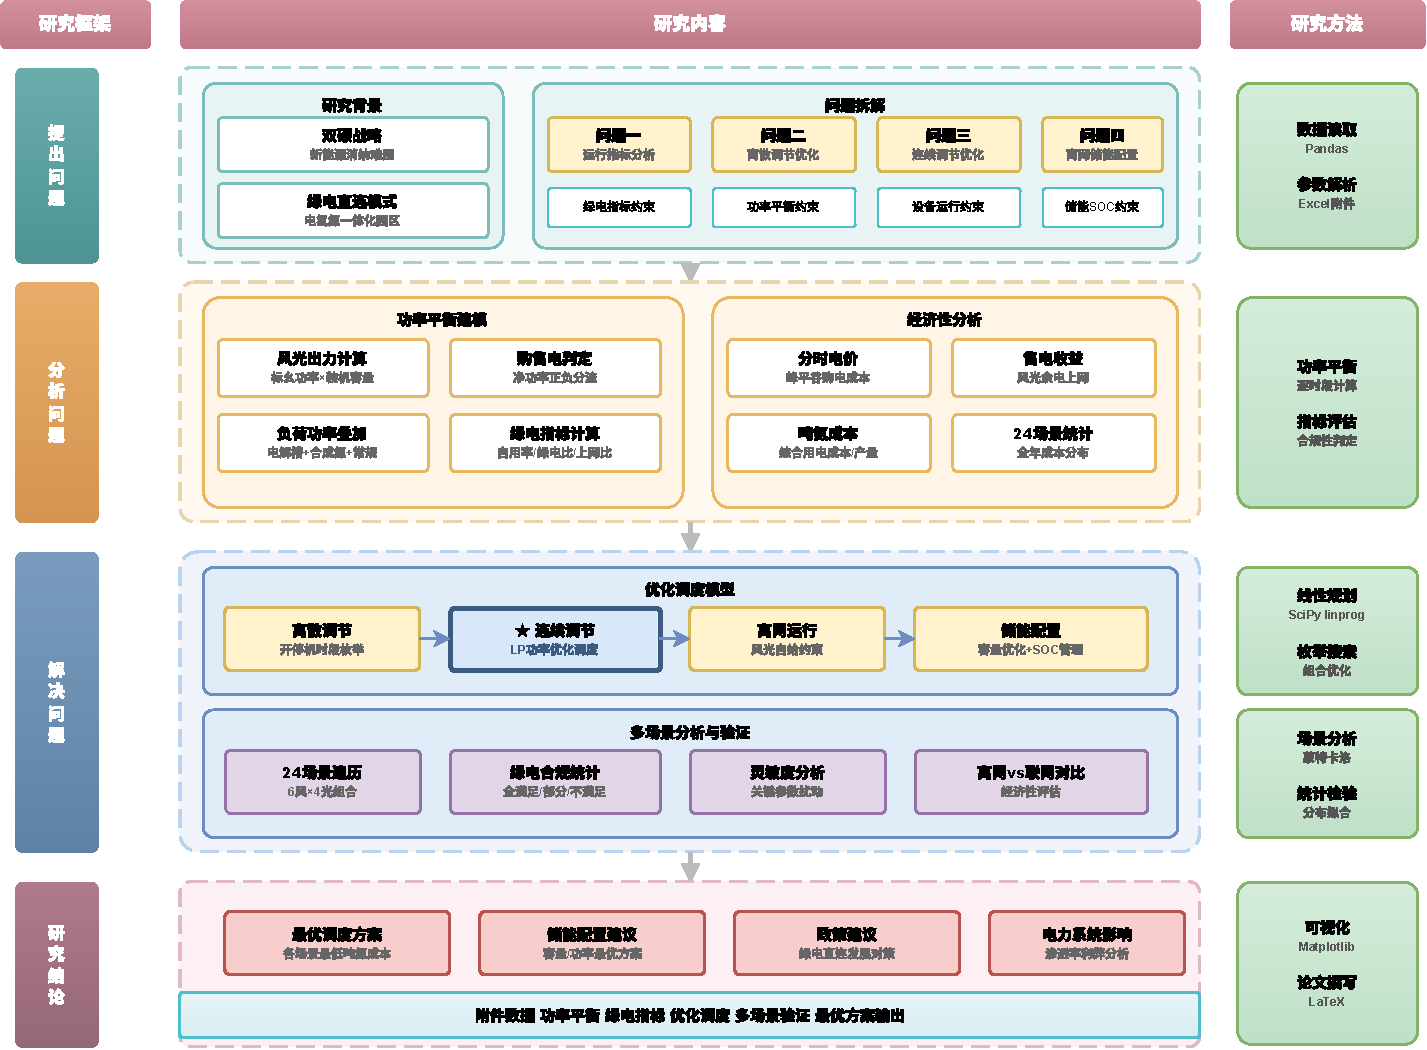
\includegraphics[width=\textwidth,height=0.45\textheight,keepaspectratio]{../figures/fig_roadmap.pdf}
\caption{整体技术路线图}\label{fig:roadmap}
\end{figure}

本文围绕上述四个问题，建立了功率平衡模型、整数线性规划模型、连续优化调度模型和两层储能配置优化模型，综合运用贪心算法、线性规划和网格搜索等方法进行求解，并通过灵敏度分析验证模型的稳健性。整体技术路线如图\ref{fig:roadmap}所示。
